\documentclass{article}
\usepackage{graphicx}

\setlength{\parindent}{0pt}
\setlength{\parskip}{5pt}

\begin{document}

\title{UADE 2.xx design specification}
\author{Heikki Orsila $<$heikki.orsila@iki.fi$>$}
\date{}
\maketitle

\section{History}

UADE 1.xx was written to be a stand-alone program that had separate code
for each possible \emph{frontend} (\emph{user interface}), but there was
no internal structure to implement different frontends easily. By much
hacking some kind of pseudo-interface was created to facilitate following
frontends:
\begin{itemize}
  \item Beep Media Player
  \item MorphOS shell without interaction
  \item Unix shell without interaction
  \item Unix shell with small interaction
  \item XMMS plugin
\end{itemize}

It was a clear design problem that needed to be fixed. To force the separation
of frontend and \emph{uadecore} (emulator), UADE 2.xx removed all user
interface issues from the uadecore.

\section{Message-passing protocol}
In UADE 2.xx the emulator (uadecore) became an independent process without
any user interfaces. Any frontend, or client, that wants to use its services
must communicate with the uadecore by using a token-passing based messaging
protocol. The protocol is of course implemented by interprocess communication
(IPC).

The basic idea of the protocol is that the frontend is the client
who issues commands for the server (uadecore). Uadecore may not send any
commands at all. Uadecore only sends replies to commands issued by the
client. Also, the client never replies anything back to the
uadecore.

The communication protocol is based on the concept of
\emph{tokens}. Only the party that has a token (there is only one) may
send messages. Messages are either commands or replies. Client sends
messages and uadecore sends replies. Both of them have to send the token back
sometimes. The party that doesn't have the token must reply to all commands
sent by the other party.

Initially the client has the token so it may send commands for the uadecore.

\subsection{Messaging protocol commands}

The messaging protocol has following commands which are only sent by
the client. There is an exception, however. The uadecore may send a
\emph{token}-command, but it is not really considered a command.
All the commands can be found from the file \mbox{src/include/uademsg.h}.

\begin{description}
\item [Config] command is used to pass a file name of the emulation
configuration file for the uadecore. The file is named \emph{uaerc}.

\item [Score] command is used to pass file name of a binary run-time in M68k
machine language for the uadecore. The binary run-time is called
\emph{score} or \emph{sound core}. The sound core contains implementations of
\emph{Eagleplayer} and \emph{AmigaOS} APIs.

\item [Player] command is used to pass a file name of a binary player plugin
in M68k machine language for the uadecore. This is also called an
\emph{Eagleplayer plugin}.

\item [Module] command is used to pass a file name of a song to be played
for the uadecore.

\item [Read] command is used to request more sound data from the uadecore.

\item [Reboot] command is used to halt playback synthesis of uadecore.

\item [Set subsong] command is used to set the initial subsong for playback.

\item [Ignore check] command is not necessary (will be documented later,
if ever).
\item [Song end not possible] command is not necessary.
\item [Set ntsc] command is not necessary.
\item [Filter] command is not necessary.
\item [Set interpolation mode] command is not necessary.
\item [Speed hack] command is not necessary.
\item [Change subsong] command is not necessary.
\item [Activate debugger] command is not necessary.

\item [Token] command is used to pass back the token for the other party.
\end{description}

\subsection{Messaging protocol replies for commands}

Messages are answered by following replies.
All the replies can be found from the file \mbox{src/include/uademsg.h}.

\begin{description}
\item [MSG] reply is just any random text string message that the client should
know. Could be spam, blackmailing, empty threats or last words of a dying
process.
\item [Can't play] reply is issued by the uadecore if it is not able to play
a given triplet of score, player and module.
\item [Can play] reply is issued by the uadecore if it can play a given
triplet of score, player and module.
\item [Song end] reply is issued by the uadecore to indicate that playback
has ended.
\item [Subsong info] is issued by the uadecore when it knows the amount of
subsongs contained in the song. This happens a short while after playback
has started, or usually during the first fraction of a second since
playback has been started.
\item [Player name] is a reply containing the human (geek?) readable player
name that is decoded by the eagleplayer plugin,
\item [Module name] is a reply containing the human readable form of the
module name decoded by the eagleplayer plugin.
\item [Format name] is a reply containing the human readable form
of the song format that is being played.
\item [Data] reply is issued by the uadecore to pass synthesized sample
data back to the client. This is a reply for the \emph{read}-command.
\end{description}.

\subsection{Message format}
All messages are sent as finite sized byte sequences. Each message begins
with a header shown in Table \ref{tab:message_header}.
\textbf{msgtype} field is simply an unsigned 32-bit integer in a packed
binary structure. The integer is sent in network byte-order aka big-endian
format. All integers are sent in big-endian format.
The \textbf{size} field is 32-bit length of the bytes coming after the header
(which is in big-endian format).
Notice the use of C99 empty record in a structure (excuse the annoying GCC
feature there that forces the structure to be tightly packed) called
\textbf{data}. \textbf{data} has zero
size and thus the whole message size in memory is $8 + size$ bytes. The
full size must not be over $4096$ bytes, and thus \textbf{size} can be
at most $4088$.

There are 3 types of messages: short messages, string messages and custom
messages. Each follow the given low-level format but the contents differs.

Messages C language definition is:
\begin{verbatim}
struct uade_msg {
  uint32_t msgtype;
  uint32_t size;
  uint8_t data[];
} __attribute__((packed));
\end{verbatim}


\begin{table}
\begin{center}
\caption{Messages header}
\label{tab:message_header}
\begin{tabular}{|r|l|}
\hline
\textbf{uint32\_t} & msgtype (big-endian) \\
\hline
\textbf{uint32\_t} & size (big-endian)\\
\hline
\textbf{uint8\_t[]} & data \\
\hline
\end{tabular}
\end{center}
\end{table}

\subsubsection{Short message}

Short message has the value $0$ in \textbf{size} field implying that there is
no special payload with the message. Sending a token, for example, is such
a message. Short messages are sent with \textbf{uade\_send\_short\_message}
and received with \textbf{uade\_receive\_short\_message}. The structure
of short message is shown in Table \ref{tab:short_message}.
Table \ref{tab:short_messages} shows all short messages.

\begin{table}
\begin{center}
\caption{Short message}
\label{tab:short_message}
\begin{tabular}{|r|l|}
\hline
\textbf{uint32\_t} & msgtype\\
\hline
\textbf{uint32\_t} & 0 \\
\hline
\end{tabular}
\end{center}
\end{table}

\begin{table}
\begin{center}
\caption{Short messages}
\label{tab:short_messages}
\begin{tabular}{|r|l|}
\hline
Command & Activate debugger\\
\hline
Command & Ignore check\\
\hline
Command & Reboot \\
\hline
Command & Song end not possible \\
\hline
Command & Speed hack \\
\hline
Command & Token \\
\hline
Reply & Can play\\
\hline
Reply & Can't play\\
\hline
\end{tabular}
\end{center}
\end{table}

\subsubsection{String message}

String message is a message containing one zero-terminated text string.
A string message is sent by \textbf{uade\_send\_string} and received by
\textbf{uade\_receive\_string}. Table \ref{tab:string_message} shows
the structure of a string message. Table \ref{tab:string_messages} shows
all string messages.

\begin{table}
\begin{center}
\caption{String message}
\label{tab:string_message}
\begin{tabular}{|r|l|}
\hline
\textbf{uint32\_t} & msgtype\\
\hline
\textbf{uint32\_t} & $x + 1$, where \textbf{x} is the number of letters.\\
\hline
\textbf{uint8\_t[]} & $x + 1$ bytes.\\
\hline
\end{tabular}
\end{center}
\end{table}

\begin{table}
\begin{center}
\caption{String messages}
\label{tab:string_messages}
\begin{tabular}{|r|l|}
\hline
Command & Config\\
\hline
Command & Module\\
\hline
Command & Player\\
\hline
Command & Score\\
\hline
Command & Set interpolation mode\\
\hline
Reply & Format name\\
\hline
Reply & Module name\\
\hline
Reply & MSG\\
\hline
Reply & Player name\\
\hline
\end{tabular}
\end{center}
\end{table}

\subsubsection{Custom message}

Custom message is any kind of message which is not short or string message.
We quickly present all different custom messages in following tables.

Table \ref{tab:reply_data} shows format of sound data reply message.
Table \ref{tab:reply_subsong_info} shows format of subsong info reply message.
Table \ref{tab:reply_song_end} shows format of song end reply message.
Table \ref{tab:command_read} shows format of read command message.
Table \ref{tab:command_filter} shows format of filter command message.
Table \ref{tab:command_subsong} shows format of subsong command messages
which are set subsong and change subsong.

\begin{table}
\begin{center}
\caption{Data reply message}
\label{tab:reply_data}
\begin{tabular}{|r|l|}
\hline
\textbf{uint32\_t} & Reply: Data \\
\hline
\textbf{uint32\_t} & $x$, where \textbf{x} is the number of sample
data bytes.\\
\hline
\textbf{uint8\_t[]} & $x$ sample data bytes. The format is 16-bit interleaved\\
& PCM stereo (big-endian).\\
\hline
\end{tabular}
\end{center}
\end{table}

\begin{table}
\begin{center}
\caption{Subsong info reply message}
\label{tab:reply_subsong_info}
\begin{tabular}{|r|l|}
\hline
\textbf{uint32\_t} & Reply: Subsong info \\
\hline
\textbf{uint32\_t} & 12\\
\hline
\textbf{uint32\_t} & Minimum subsong (big-endian)\\
\hline
\textbf{uint32\_t} & Maximum subsong (big-endian)\\
\hline
\textbf{uint32\_t} & Current subsong (big-endian)\\
\hline
\end{tabular}
\end{center}
\end{table}

\begin{table}
\begin{center}
\caption{Song end reply message}
\label{tab:reply_song_end}
\begin{tabular}{|r|l|}
\hline
\textbf{uint32\_t} & Reply: Song end\\
\hline
\textbf{uint32\_t} & $8 + x + 1$, where \textbf{x} is length of an explanation string.\\
\hline
\textbf{uint32\_t} & Number of bytes of sample data valid in the next data reply (big-endian)\\
\hline
\textbf{uint32\_t} & Unintentional end: 0 or 1. 0 means unintentional.\\
 & 1 means an error resulted into the song end. (big-endian)\\
\hline
\textbf{uint8\_t[]} & $x + 1$ bytes containing a textual reason for song end.\\
\hline
\end{tabular}
\end{center}
\end{table}

\begin{table}
\begin{center}
\caption{Read command message}
\label{tab:command_read}
\begin{tabular}{|r|l|}
\hline
\textbf{uint32\_t} & Command: Read\\
\hline
\textbf{uint32\_t} & 4\\
\hline
\textbf{uint32\_t} & Number of bytes of sample data to be read (big-endian)\\
\hline
\end{tabular}
\end{center}
\end{table}

\begin{table}
\begin{center}
\caption{Filter command message}
\label{tab:command_filter}
\begin{tabular}{|r|l|}
\hline
\textbf{uint32\_t} & Command: Filter\\
\hline
\textbf{uint32\_t} & 8\\
\hline
\textbf{uint32\_t} & Filter type. See \mbox{src/include/amigafilter.h} for values (big-endian).\\
\hline
\textbf{uint32\_t} & $2x+y$, where \textbf{x} means whether or not filter state should be forced\\
 & and \textbf{y} is filter state to be set. Both $x$ and $y$ are either 0 or 1. (big-endian)\\
\hline
\end{tabular}
\end{center}
\end{table}

\begin{table}
\begin{center}
\caption{Subsong command message}
\label{tab:command_subsong}
\begin{tabular}{|r|l|}
\hline
\textbf{uint32\_t} & Command: change subsong or set subsong\\
\hline
\textbf{uint32\_t} & 4\\
\hline
\textbf{uint32\_t} & New subsong number (big-endian).\\
\hline
\end{tabular}
\end{center}
\end{table}

\section{Interaction example}

To illustrate the dialog between client and server, look at the following log
between uade123 and uadecore:
\begin{verbatim}
<This is done once during client startup>
uade123: sending string 1 (command: config)

<Here begins play back of new song. this is done for each song.>
uade123: sending string 2 (command: score)
uade123: sending string 3 (command: player)
uade123: sending string 4 (command: module)
uade123: sending message 16 (token pass)

<Now the uadecore is pondering whether or not the thing can be played>
uadecore: sending message 19 (reply: can play)
uadecore: sending message 16 (token pass back)

<It's okay to play, so send some additional commands for uadecore>
uade123: sending message 11 (command: filter. not needed.)
uade123: sending string 12 (command: interpolation. not needed.)

<Then start audio synthesis by issuing read command>
uade123: sending message 5 (command: read)
uade123: sending message 16 (token pass)

<uadecore starts to synthesize and floods back messages>
uadecore: sending string 17 (reply: message. don't care.)
uadecore: sending string 22 (reply: player name back. don't care.)
uadecore: sending string 23 (reply: module name back. don't care.)
uadecore: sending message 21 (reply: subsong info)
uadecore: sending string 17 (reply: birthday congratulation message)
uadecore: sending message 25 (reply: data)
uadecore: sending message 25 (reply: data)
uadecore: sending message 16 (token back as all the requested data has been sent)

<Okay, the first round of messages was good. Next read then..>
uade123: sending message 5 (command: read. 2nd one actually.)
uade123: sending message 16 (token pass)
uadecore: sending message 25 (reply: data)
uadecore: sending message 25 (replay: data)
...
\end{verbatim}

Based on that log and previous explanation of messages, you should be able
to write an independent frontend by doing little reverse-engineering into
uade headers. More specifically, you need following information:
\begin{itemize}
\item Message type numbers (see \mbox{src/include/uademsg.h})
\item Filter setting codes (see \mbox{src/include/amigafilter.h})
\item something else you will find out..
\end{itemize}

Figure \ref{fig:playloop} shows play loop interaction from client
perspective. That is, song initialization has already happened which means
that uadecore configuration, score, player and module names and other
options have been sent already.

\begin{figure}
\centering
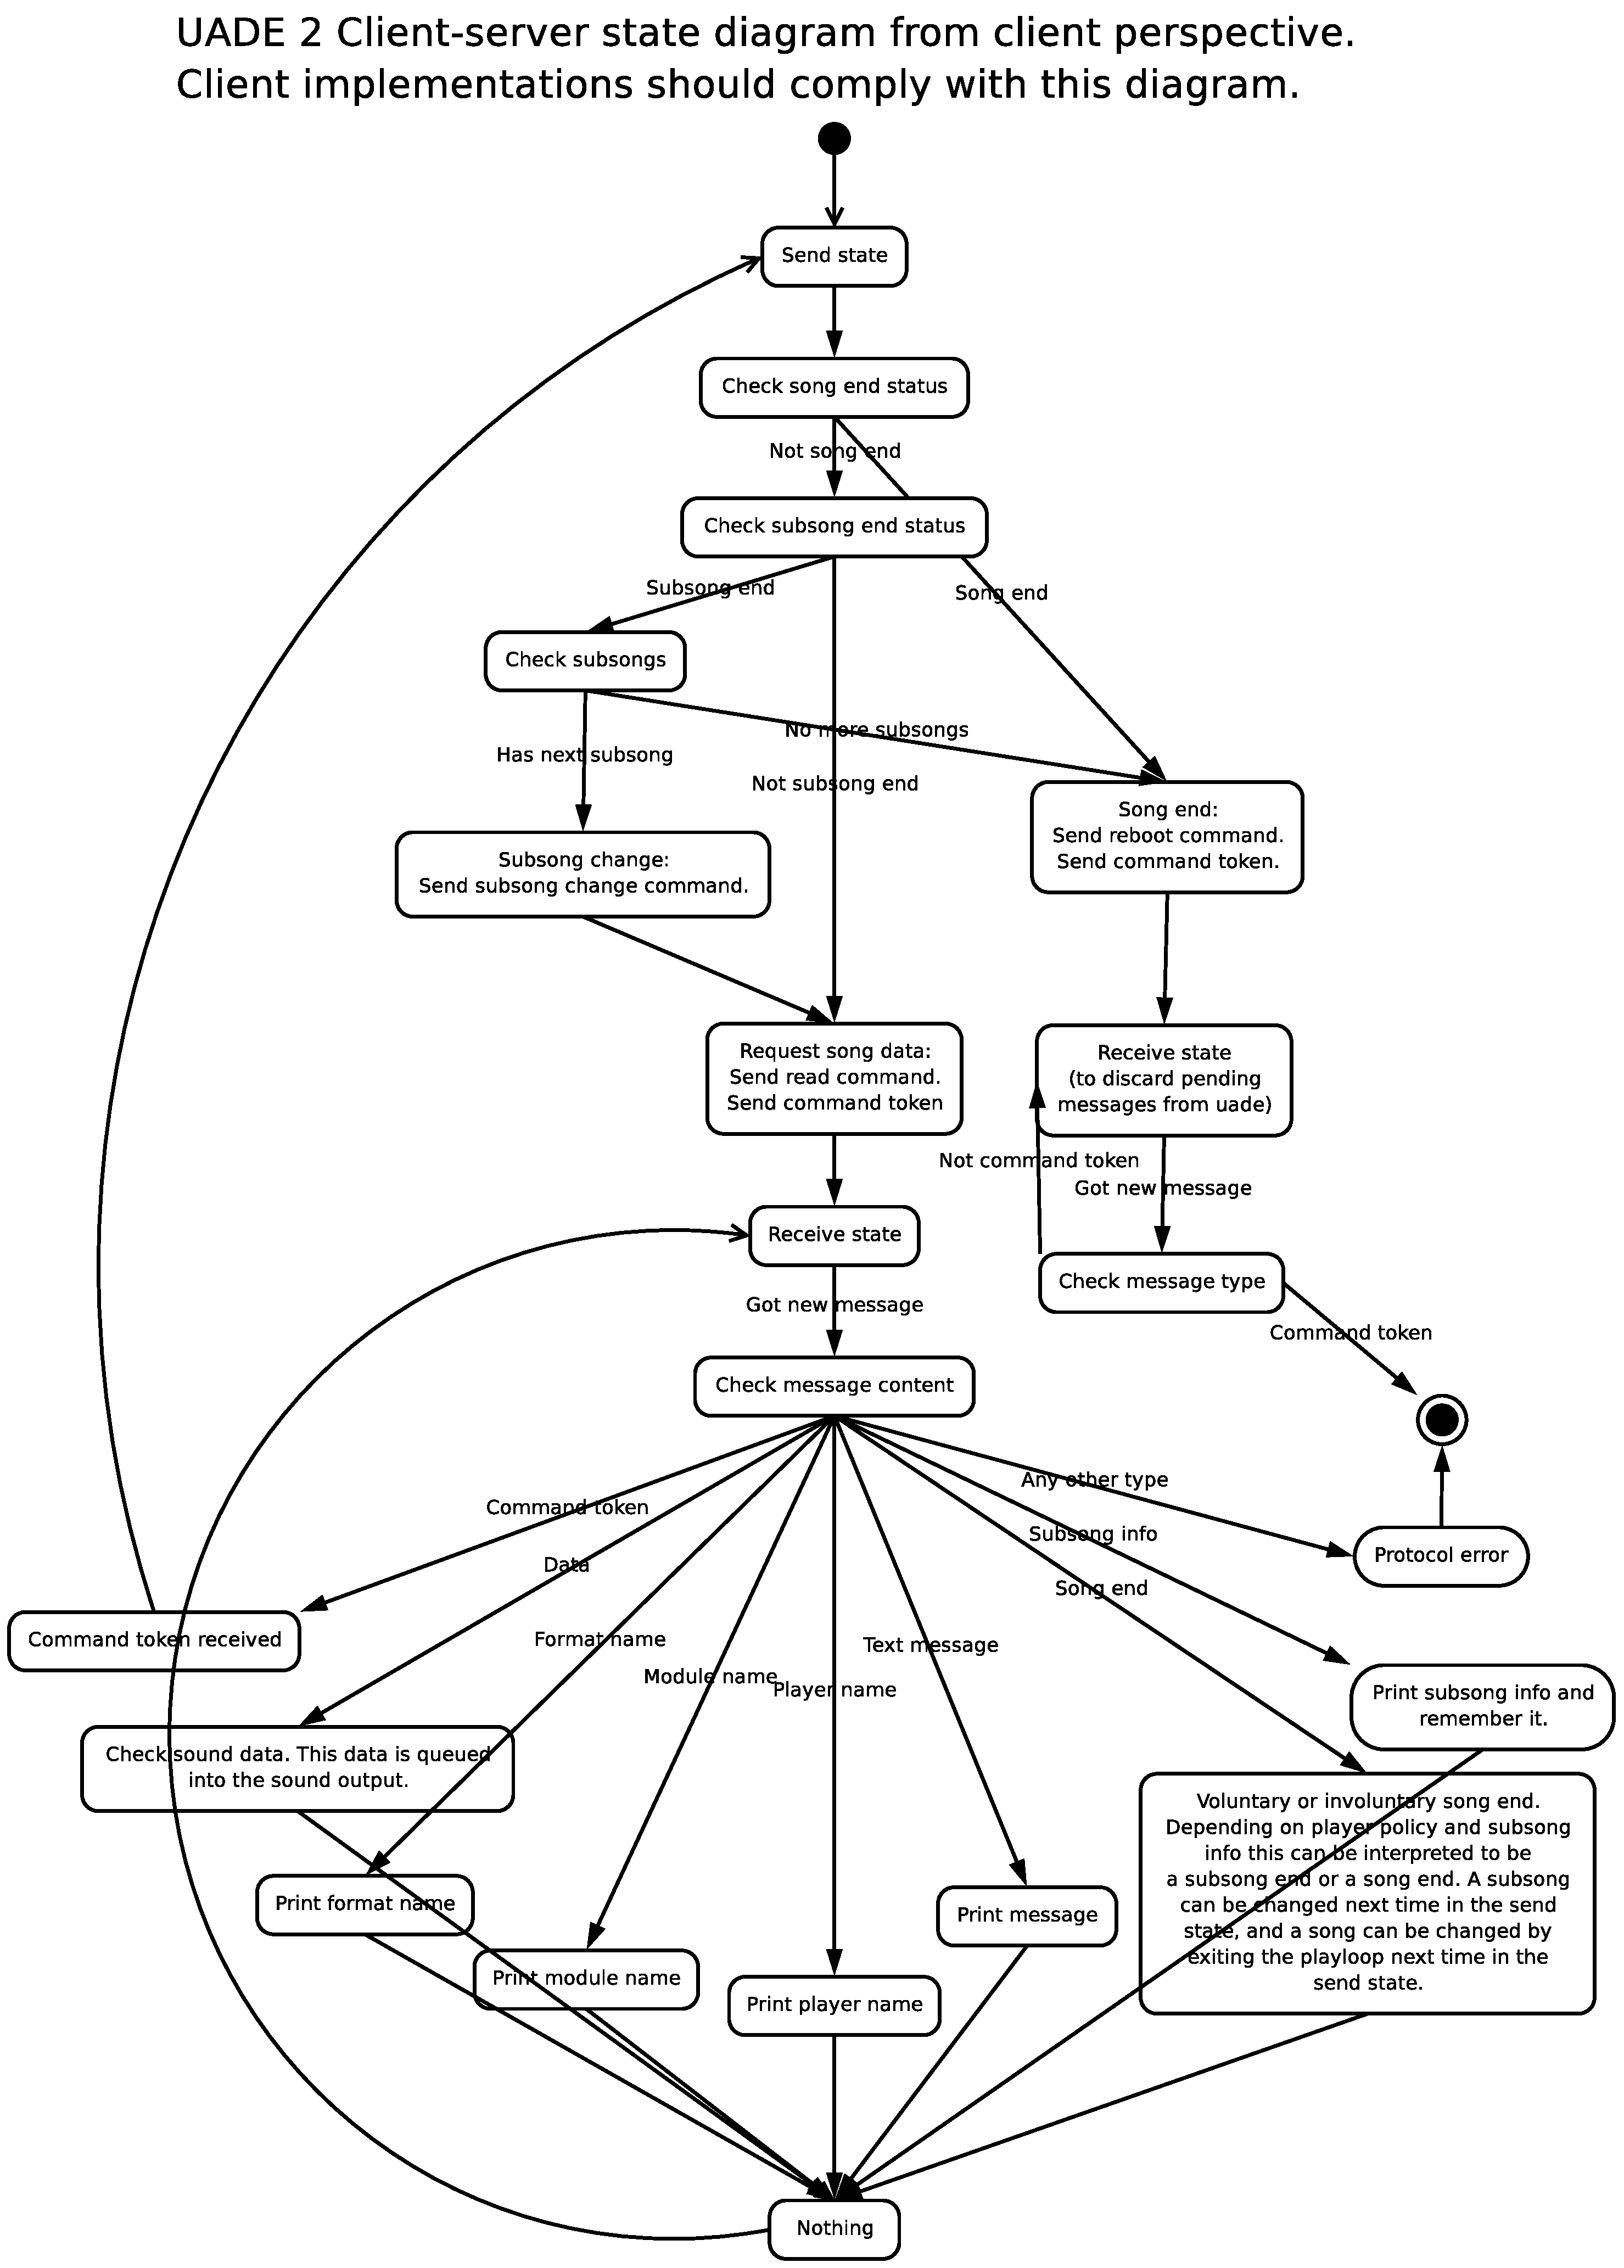
\includegraphics[scale=0.25]{play_loop_state_diagram.eps}
\caption{Play loop interaction from client (frontend) perspective}
\label{fig:playloop}
\end{figure}

\end{document}
